\section{Current Security of the Graphic Stack}

\begin{frame}
\frametitle{DRM: Update since our talk @ XDC2012}
	\begin{block}{Drivers: Per-process virtual address space}
		\begin{itemize}
			\item Intel: WIP; Nouveau \& Radeon: done
		\end{itemize}
	\end{block}

	\begin{block}{X-Server}
		\begin{itemize}
			\item DRI3: Use DMA-Buf instead of GEM flink for BO-passing
			\item but the X protocol is still unsecure \textbf{by design}...
		\end{itemize}
	\end{block}

	\begin{block}{Wayland/Weston}
		\begin{itemize}
			\item Designed with security in mind from the ground up
			\item now uses DMA-Buf instead of GEM-flink to provide client isolation
			\item relies on DRM drivers for its security
		\end{itemize}
	\end{block}
\end{frame}

\begin{frame}
\frametitle{But How to Build a Secure OS?}

	\begin{block}{Some critical concepts}
	\begin{enumerate}[leftmargin=1.6em]
	\item[Complete Mediation] Requires client isolation in the HW, kernel, the display server \textit{and} sandboxing
	\item[Least Privilege] Need for mandatory security within user sessions	and means to identify privileged clients
	\item[Trusted Path] Unspoofable ways for user and trusted apps to communicate; Allows reading the user's intent
	\end{enumerate}
	\end{block}

	All of the above needed to prevent evil apps from hurting you!
	{\scriptsize\color{xorg-palette-dark}\cite{saltzer_protection_1975,loscocco_inevitability_1998}}
	%Economy of Mechanism, Fail-safe Defaults, Open Design, Psychological Acceptability

\end{frame}

\begin{frame}
\frametitle{Challenges of creating a secure Desktop 1/2}

	\begin{block}{Some common GUI requirements are un-secure by design}
		\begin{itemize}
			\item Clipboard monitoring
			\begin{itemize}
				\item Acceptable: check that data can be pasted (for GUI toolkits)
				\item Unacceptable: access sensitive data
			\end{itemize}
			\item Key events monitoring
			\begin{itemize}
				\item Acceptable: global hotkeys
				\item Unacceptable: keylogging, reading your passwords
			\end{itemize}
			\item Input-injection
			\begin{itemize}
				\item Acceptable: visual keyboards / accessibility
				\item Unacceptable: command injection
			\end{itemize}
		\end{itemize}
	\end{block}

% TODO
% 	Clipboard spying (ref android sacha fohl)
% 	Keylogging (ref qubes but many other methods) and command injection (ref myself for poc)
% 	Clickjacking (focus raise, mouse)
% 	Auth UI spoofing (fullscreen)

\end{frame}

\begin{frame}
\frametitle{Challenges of creating a secure Desktop 2/2}

	\begin{block}{}
		\begin{itemize}
			\item Focus raising
			\begin{itemize}
				\item Acceptable: show apps requiring user input before a power down
				\item Unacceptable: window stealing the user's input while authenticating
			\end{itemize}
			\item Full-screen support
			\begin{itemize}
				\item Acceptable: video, gaming, full-screen shell
				\item Unacceptable: spoofing the greeter
			\end{itemize}
		\end{itemize}
	\end{block}

	\begin{block}{Solutions by the X-Server vs Wayland/Weston}
		\begin{itemize}
			\item X-Server: One valid use case $\rightarrow$ access granted to everyone
			\item Wayland: One invalid use case $\rightarrow$ access denied to everyone
		\end{itemize}
	\end{block}
\end{frame}

\begin{frame}
\frametitle{Current solution on Wayland/Weston}
	\begin{block}{Wayland's privileged interfaces:}
		\begin{itemize}
			\item Not defined yet, many discussions
			\item partially due to the security implications
			\item the compositor sometimes need the user intent (Trusted Path)
			\item users or packagers may want to work around that!
		\end{itemize}
	\end{block}

	\begin{block}{Example: Wayland/Clipboard}
		Reading the clipboard doesn't seem to be defined. Drag \& Drop is however supported
		because the compositor gets the user's intent!
	\end{block}
\end{frame}

\begin{frame}
\frametitle{Example of policies for accessing a privileged iface}
	\begin{center}
		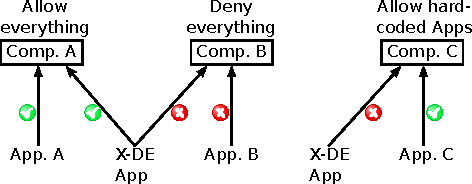
\includegraphics[width=\linewidth]{figures/libwsm_without.pdf}
	\end{center}
\end{frame}

\begin{frame}
\frametitle{Challenges of defining policies}
	\begin{block}{Challenges of defining policies}
		\begin{itemize}
			\item Many Desktop Environments (Gnome, KDE, Tizen, XFCE, etc...)
			\item DEs won't agree on a single policy
			\item Cross-DE apps cannot ship with a policy for every DE
			\item Packagers need a simple policy interface
		\end{itemize}
	\end{block}

	\begin{block}{Possible solution?}
		\begin{itemize}
			\item Abstract the decision process in a multi-backend library
			\item Create a generic policy and per-DE tweaks
		\end{itemize}
	\end{block}
\end{frame}

% Not everyone will agree on policies and methods to manage security between KDE,GNOME,XFCE,Tizen,etc.
% And yet app developers can't ship a profile per OS/DE combination
% App packagers probably need something much simpler than e.g. SELinux policies
% Windows, OS X, Android, iOS all use capabilities to describe what apps can do
% When it comes to GS capabilities there are relatively few differences in what's available among DEs
% Only the policies may really change
% Things like menu management or autostarting only on some DEs work
% Why not do the same for capability permissions? Generic policies and DE customisation
% Can we build a capability infrastructure that can be used and extended by all DEs without limits?

\section{Introducing Wayland Security Modules}
\begin{frame}
\frametitle{Wayland Security Modules}
	
	\begin{block}{Goals}
	\begin{itemize}
	\item Provide security decisions for Wayland privileged ifaces
	\item Help DEs store policy for their ifaces in a centralised way
	\item Support innovation and standardisation over time
	\end{itemize}
	\end{block}

	\begin{block}{How we do that}
	\begin{itemize}
	\item Hooks on all privileged ifaces in the Wayland API
	\item Support for any backend/module: just a few symbols to export
	\item Simple: currently about 1100 LOCs w/ default backend
	\item Very extensible!
	\end{itemize}
	\end{block}

\end{frame}

\begin{frame}
\frametitle{Example of policies for accessing a privileged iface}
	\begin{center}
		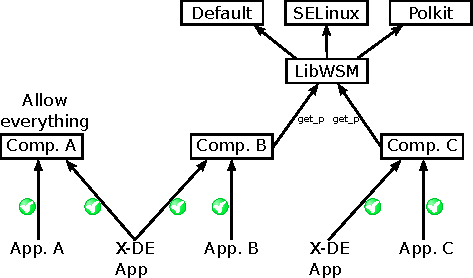
\includegraphics[width=\linewidth]{figures/libwsm_with.pdf}
	\end{center}
\end{frame}

\begin{frame}
\frametitle{How to Use}

	\begin{block}{Modifications to a compositor}
	\begin{enumerate}
	\item \texttt{wsm\_init()} on compositor start
	\item \texttt{wsm\_new\_client()} on new client	
	\item Users choose a backend and write a policy -- or use ours!
	\item When implementing privileged ifaces, call \texttt{wsm\_get\_permission()}
	\item Got custom semantics? Call \texttt{wsm\_get\_custom\_permission()}
	\item \texttt{wsm\_client\_free()} and \texttt{wsm\_fini()} to clean up
	\end{enumerate}
	\end{block}

	\begin{block}{Source}
		\url{https://github.com/mupuf/libwsm}
	\end{block}

\end{frame}

\begin{frame}
\frametitle{LibWSM Security Decisions 1/2}

	\begin{block}{Four default semantics}
	\begin{enumerate}[leftmargin=1em]
	\item[Allow] Client explicitly allowed use of a privileged iface.
	\item[Soft Allow] Client allowed, but there could be issues. We recommend notifying the user.
	\item[Soft Deny] Client denied, but no particular concern. You could grant access via trusted UIs or prompts. 
	\item[Deny] Client explicitly denied by policy, don't proceed.
	\end{enumerate}
	\end{block}

	If LibWSM answers something else, implement {\color{xorg-palette-light}Deny}.
	
	If there is no policy, the default backend will reply {\color{xorg-palette-light}Soft Deny}.
\end{frame}

\begin{frame}
\frametitle{LibWSM Security Decisions 2/2}

	\begin{block}{Why the distinction?}
	\begin{enumerate}[leftmargin=1em]
	\item[Hard decisions] represent the actual security policy. Please respect it.
	\item[Soft decisions] are assumptions about what's best. Compositors can probably do better than just allow/deny.
	\end{enumerate}
	\end{block}
	
	Security notifications, Trusted UIs, User-driven access control and Permission prompts should come to mind with soft replies.

\end{frame}

\begin{frame}[fragile]
\frametitle{Extending LibWSM is Easy!}
	
	\begin{block}{Support for custom capabilities...}
	Compositors should be let to innovate securely: custom ifaces like \texttt{\_WESTON\_FULLSCREEN} can be mediated.
	\end{block}
	
	\begin{block}{Custom decision semantics...}
	If you implement specific behaviours, you can express them in the policy \textit{e.g.},
	``allow if no sensitive apps open'' for \texttt{WSM\_SCREENSHARING}.
	\end{block}

	\begin{block}{Different policies per compositor...}
	Write per-DE policies just like in menu or autostart files, e.g.:
	\begin{verbatim}
	[GNOME]
	WSM_RAISE_FOCUS=deny
	\end{verbatim}
	\end{block}
	
\end{frame}

\begin{frame}
\frametitle{LibWSM Capabilities 1/3}

	\begin{block}{\texttt{WSM\_SCREENSHOT}}
	Take a screenshot of the whole screen {\small({\color{xorg-palette-light}Soft Deny})}
	\end{block}

	\begin{block}{\texttt{WSM\_SCREENSHARING}}
	Record the screen continuously ({\color{xorg-palette-light}Soft Deny})
	\end{block}

	\begin{block}{\texttt{WSM\_VIRTUAL\_KEYBOARD}}
	Inject or filter input events on keyboard ({\color{xorg-palette-light}Soft Deny})
	\end{block}

	\begin{block}{\texttt{WSM\_VIRTUAL\_POINTING}}
    Modify the position of the pointer and simulate clicks ({\color{xorg-palette-light}Soft Deny})
	\end{block}
\end{frame}

\begin{frame}
\frametitle{LibWSM Capabilities 2/3}
	\begin{block}{\texttt{WSM\_FULLSCREEN}}
	Use the entire screen ({\color{xorg-palette-light}Soft Allow})
	\end{block}

	\begin{block}{\texttt{WSM\_GLOBAL\_KEYBOARD\_SEQUENCE} {\fontseries{sb}\color{xorg-slide-fg}{\scriptsize[obj: key sequence]}}}
	Receive keyboard sequences even when not active ({\color{xorg-palette-light}Soft Deny})
	\end{block}

	\begin{block}{\texttt{WSM\_FORWARD\_RESERVED\_KEYBOARD\_SEQUENCE} {\fontseries{sb}\color{xorg-slide-fg}{\scriptsize[obj: key sequence]}}}
	Receive reserved compositor sequences when active ({\color{xorg-palette-light}Soft Deny})
	\end{block}

	\begin{block}{\texttt{WSM\_RAISE\_FOCUS}}
	Raise the window and grab focus programmatically
	({\color{xorg-palette-light}Soft Allow})
	\end{block}
\end{frame}

\begin{frame}
\frametitle{LibWSM Capabilities 3/3}
	\begin{block}{\texttt{WSM\_CLIPBOARD\_COPY}}
	Copy programmatically to the clipboard ({\color{xorg-palette-light}Allow})
	\end{block}

	\begin{block}{\texttt{WSM\_CLIPBOARD\_PASTE}}
	Paste from the clipboard ({\color{xorg-palette-light}Soft Deny})
	\end{block}
	
	\vspace{1.5em}
	
	\begin{important}
	Of course this list is provisional. Please suggest corrections/additions
	at \url{https://github.com/mupuf/libwsm/issues}.
	\end{important}
	
	\vspace{3em}
\end{frame}


\begin{frame}
\frametitle{The Default Backend}

	\begin{block}{Policy managed with files}
	\begin{itemize}
	\item default policy, app-specific policies, policy templates (WIP)
	\item system-wide policies can be customised by users
	\end{itemize}
	\end{block}

	\begin{block}{A single source of policy per app at any time}
	\begin{itemize}
	\item more manageable for packagers and distributions
	\item better visibility (includes in SELinux are a recipe for trouble)
	\end{itemize}
	\end{block}
\end{frame}


\begin{frame}[fragile]
\frametitle{Example Default Policy}

\tiny
	\begin{verbatim}
[Wayland Security Entry]
Exec=*
Version=1

[All Compositors]
WSM_FULLSCREEN=soft-allow
WSM_CLIPBOARD_COPY=allow
WSM_RAISE_FOCUS=soft-allow

[Paranoid Shell]
WSM_FULLSCREEN=deny
WSM_CLIPBOARD_COPY=deny

[GNOME]
_GNOME_USE_SHELL_API=basic-access

[Mupuf]
WSM_FULLSCREEN=soft-allow
_WESTON_FULLSCREEN=soft-allow

[Weston]
_WESTON_FULLSCREEN=implicit-deny
	\end{verbatim}
\normalsize

\end{frame}


\begin{frame}[fragile]
\frametitle{Example Policy for an Application}

\tiny
	\begin{verbatim}
[Wayland Security Entry]
Exec=/usr/bin/example
Version=1

[All Compositors]
WSM_FULLSCREEN=allow
WSM_CLIPBOARD_COPY=deny

[Paranoid Shell]
WSM_FULLSCREEN=deny
WSM_CLIPBOARD_COPY=deny

[GNOME]
_GNOME_USE_SHELL_API=allow

[Mupuf]
WSM_FULLSCREEN=allow
_WESTON_FULLSCREEN=permanent-allow-if-frequent

[Weston]
_WESTON_FULLSCREEN=allow
	\end{verbatim}
\normalsize

\end{frame}


\begin{frame}
\frametitle{This is Just a Backbone}

	We made it as flexible as possible.
	
	~

	\begin{block}{Goal: positive user experiences}
	\begin{itemize}
	\item Easy to conceptualise and edit policy, easy to add UI
	\item Soft decisions let DEs build their own UX
	\end{itemize}
	\end{block}
	
	~
	
	Need something more for your shell? Talk to us!
\end{frame}

	
	
\begin{frame}
\frametitle{Potential Security Tasks \& Interactions}

%What functions do the users need from the document?
%What information might the users need, and in what form do they need it?
  \begin{block}{GUIs might be necessary for}
  \begin{itemize}
  \item Answering an app's permission request
  \item Installing an app which needs privileges
  \item Knowing what privileges an app has
  \item Revoking an app's privileges
  \item Prevent annoying apps from requesting privileges
    \begin{itemize}
    \item {\footnotesize (``why'' may influence the design)}
    \end{itemize}
  \end{itemize}
  \end{block}

This is the job of DEs!

\end{frame}

	
	

\section{Facts and myths about humans and security}
\begin{frame}
\frametitle{Introducing my research group...}

	\begin{block}{I'm a PhD student at UCL Info Sec}
	We specialise in usable and productive security.
	\vskip0.4em
	I'm investigating how Linux users manage their security!
	\end{block}
	
	\begin{itemize}
	\item We don't know what makes security software work... yet
	\item We don't know how to change home user behaviour... yet
	\item But we know how to do user research!
	\end{itemize}

~

	Shameless advertising: \url{http://sec.cs.ucl.ac.uk}

\end{frame}

\begin{frame}
\frametitle{Some Research Knowledge 1/3}
	\begin{block}{User time is precious, respect it}
	\begin{itemize}
	\item Nobody wants to perform security tasks! People \textit{rationally} reject costly security advice
	\item Nobody has time for security! More security pressure decreases willingness to comply
	\item Most security warnings discarded in $~2s$. One reason: people habituated to warnings, but there could be others
	\end{itemize}
	\end{block}
	
	{\scriptsize\color{xorg-palette-dark}\cite{beautement_compliance_2008,herley_so_2009,krol_dont_2012,akhawe_alice_2013}}
\end{frame}


\begin{frame}
\frametitle{Some Research Knowledge 2/3}
	\begin{block}{Security is desirable}
	\begin{itemize}
	\item People in corporate want insecure options \textit{hidden by default}
	\item They still bypass or disable security to get stuff done
	\item And still deploy their own security strategies to compensate
	\end{itemize}
	\end{block}

	{\scriptsize\color{xorg-palette-dark}\cite{bartsch_how_2013,kirlappos_learning_2014} + private conversations with Sasse}
\end{frame}


\begin{frame}
\frametitle{Some Research Knowledge 3/3}
	\begin{block}{Home users are not very concerned}
	\begin{itemize}
	\item Home users think they will never be targeted. Telling them about opportunistic criminals best triggers concern
	\item Speak of malware as medical infections, it's better understood than other metaphors
	\item Some people think antivirus software keeps them safe
	\item Linux users feel Linux is more secure (but it's not)
	\end{itemize}
	\end{block}

	{\scriptsize\color{xorg-palette-dark}\cite{camp_mental_2006,wash_folk_2010,krol_dont_2012} + market research and own observations}
\end{frame}


%\begin{frame}
%\frametitle{Some Personal Advice}
%	%FIXME
%	\begin{itemize}
%	\item \textbf{Humans are very diverse}
%	\item Interactions are not influenced only by the UI
%	\item Use \textit{interaction cost} to foster secure behaviour
%	\item Anecdotal evidence is OK to document diversity of practices, but \textit{not} for justifying decisions that prevent practices
%	\item Studies are best done in the wild, not under artificial conditions
%	\end{itemize}
%\end{frame}


\begin{frame}
\frametitle{What Makes Security Work?}

\textbf{Warning: nobody really knows!}

    \begin{block}{Some sanity principles for now:}
    \begin{enumerate}
    \item Don't put the cost of security on users!
    	\begin{itemize}
    	\item Interaction cost of security
    	\item Initial cost of \textit{`opt-in'} security
    	\item Lost features $\rightarrow$ hinders practices
    	\end{itemize}
    \item Don't ask app devs to do the security
    \item Complex policy = opaque breakdowns
    \item Test with real people as often as possible
    \end{enumerate}
    \end{block}
\end{frame}





\section{Security UIs, Infrastructure and Pitfalls to Avoid}

\begin{frame}
\frametitle{\circled{\large{1}} Trusted UIs}

  \begin{block}{What, How}
  \begin{itemize}
  \item UIs that are controlled by the OS/Compositor (not by apps)
  \item \textbf{Trusted path between Trusted UIs and user}
  \item Which means need for a UI embedding protocol
  \end{itemize}
  \end{block}

  \begin{block}{Goal}
  \begin{itemize}
  \item Indicate user intent without policy when interacted with
  {
    \scriptsize
    \begin{itemize}
    \item \scriptsize Trusted File Dialog / Power boxes~\cite{yee_aligning_2004}
    \item \scriptsize Secure ``Take Photo'' button on Android~\cite{roesner_user-driven_2012}
    \end{itemize}
  }
  \item Some Trusted UIs in Windows 8 and OS X
  \item Sadly, they require API changes in toolkits...
  \end{itemize}
  \end{block}

\end{frame}


\begin{frame}
\frametitle{PoC: File Chooser Dialog}
\framesubtitle{Remediating the Need for Filename Autocompletion}
\centering
\vspace{-0.8em}
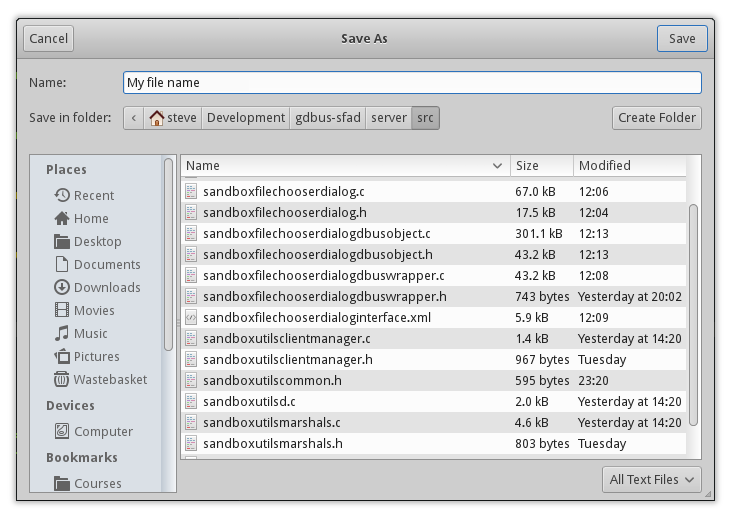
\includegraphics[height=0.85\textheight]{figures/sfcd-orig.png}
\end{frame}


\begin{frame}
\frametitle{An Initial PoC for GTK+ File Chooser Dialog}
      
  \begin{itemize}
  \item Mirror the ``normal'' usage of API: almost all apps portable
  \item Prevent attacks when user interacts w/ GUI
  \item Expose statefulness and error handling to apps
  \end{itemize}

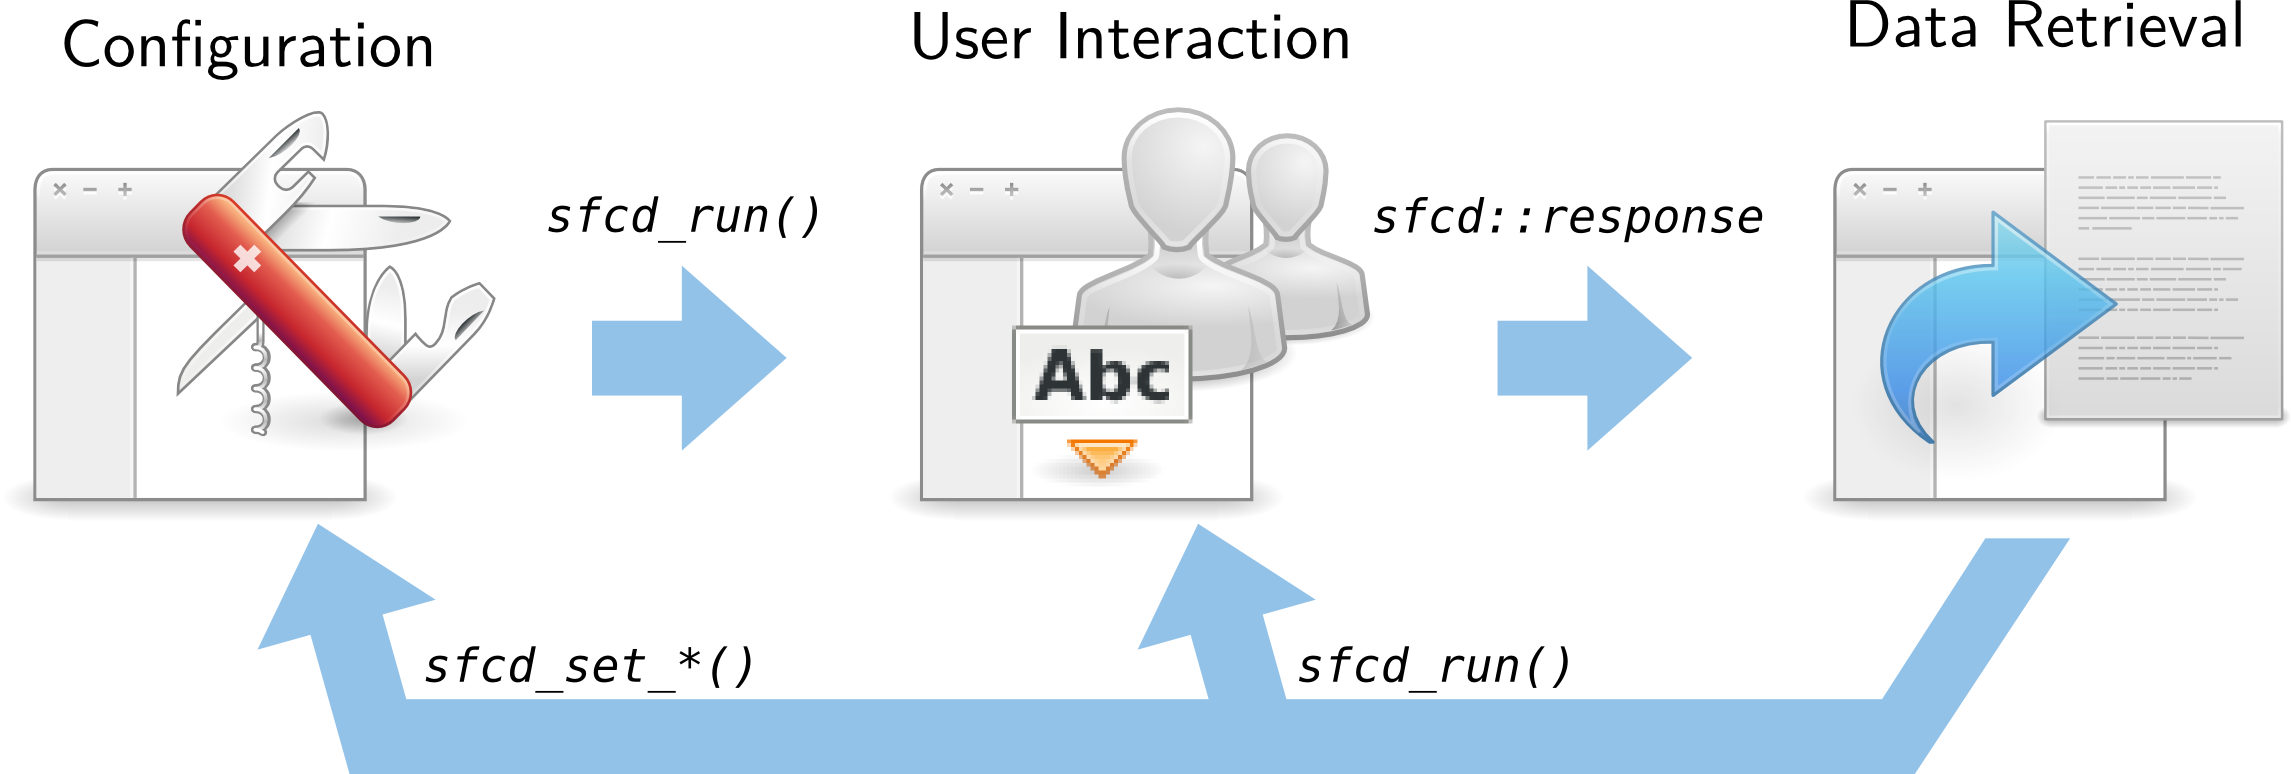
\includegraphics[height=0.45\textheight]{figures/sfcd-states.jpg}

\begin{important}
Microsoft switched to a full async programming model: no error handling when permission is denied!
\end{important}
\end{frame}


\begin{frame}
\frametitle{Is it really that simple?}

  \begin{block}{Issues arising with new FCD}
  \begin{itemize}
  \item File preview: should move to built-in DE routine
  \item \textbf{Custom widgets: needs a UI embedding protocol}
    {\scriptsize \begin{flushright}would work for apps \textbf{currently} using such widgets\end{flushright}}
  \item Autocompletion of file extension when saving?
  \end{itemize}
  \end{block}
  
  \begin{important}
  Truth is both APIs and widgets need to be redesigned.\\
  More complex workflows need entirely new UIs
  \end{important}
\end{frame}


%\begin{frame}
%\frametitle{PoC: File Chooser Dialog}
%\framesubtitle{Remediating the Need for Filename Autocompletion}
%\centering
%\vspace{-0.8em}
%\only<1>{
%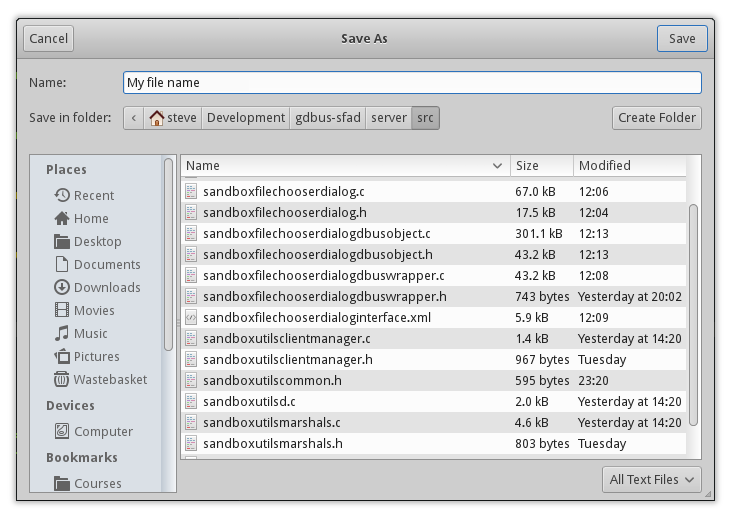
\includegraphics[height=0.85\textheight]{figures/sfcd-orig.png}
%}\only<2>{
%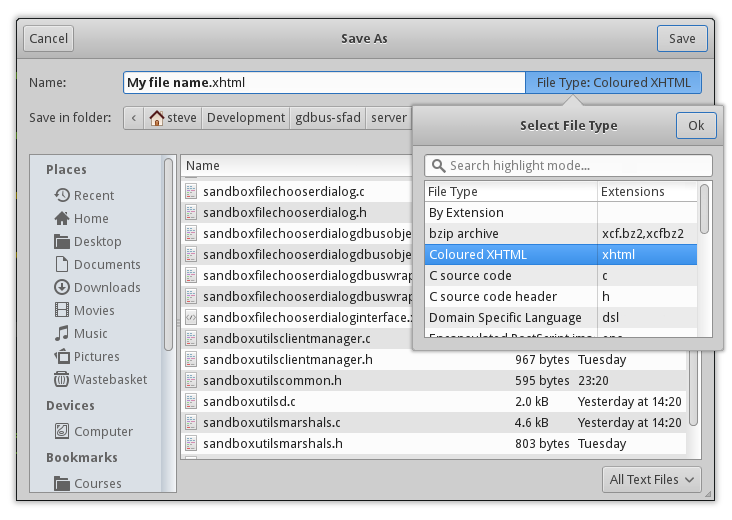
\includegraphics[height=0.85\textheight]{figures/sfcd-popover.png}
%}
%\end{frame}


\begin{frame}
\frametitle{Another Example: X11 Selections}

	\begin{block}{An actual security issue}
	\begin{itemize}
	\item Apps can paste selection content w/out mediation
	\item They routinely check if they support the content type of selections
	\end{itemize}
	\end{block}

	\begin{center}
	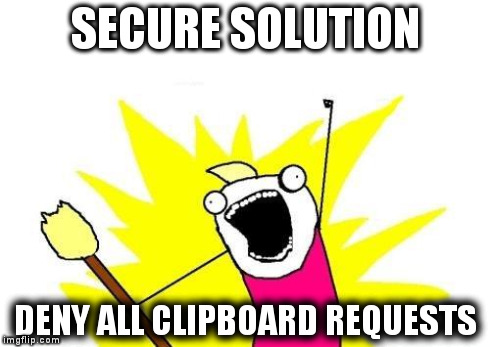
\includegraphics[height=0.55\textheight]{ban-clipboard.png}
	\end{center}

  \begin{block}{}
  \begin{itemize}
  \item Apps can paste selection content w/out mediation
  \item They routinely check if they support the content type of selections
  \item Opening/Saving groups of related files
    \begin{itemize}
    \item Playlist Opener
    \item Session Saver/Resumer
    \end{itemize}
  \item Folder Scanner
  \end{itemize}
  \end{block}
  
  \begin{important}
    GNOME Competition: Content Selection \& Sharing APIs
  \end{important}
\end{frame}


\begin{frame}
\frametitle{Is a Secure Clipboard Possible?}

  \begin{block}{Apps should receive clipboard events}
  \begin{itemize}
  \item Implication: need a reserved hotkey for pasting 
  \item And Trusted UIs buttons and menu items
	  \\\hspace{3em} 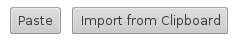
\includegraphics[height=2em]{paste-buttons.png}
  \item \textbf{We do need a (two-way) UI embedding protocol}
  \end{itemize}
  \end{block}

  \begin{block}{Risk of issues down the road}
  \begin{itemize}
  \item What about apps that use other labels/keyboard sequences?
  \item Share your concerns/critics with us, it will help!
  \end{itemize}
  \end{block}
\end{frame}



\begin{frame}
\frametitle{\circled{\large{2}} Permission Requests}

  \begin{columns}[T]
    \begin{column}{0.6\paperwidth}
    \vspace{1.2em}
    Permission requests \textbf{don't provide security.} Systematically ignored: lack of experience, disruptiveness, immediate gratification bias, \textbf{economic rationality / compliance budget}
    \end{column}
    \begin{column}{0.33\paperwidth}
      
\includegraphics[scale=0.2]{figures/pigs.png}
    \end{column}
  \end{columns}

  \begin{block}{How to ask for Permission {\fontseries{sb}{\scriptsize\cite{felt_how_2012}}}}
  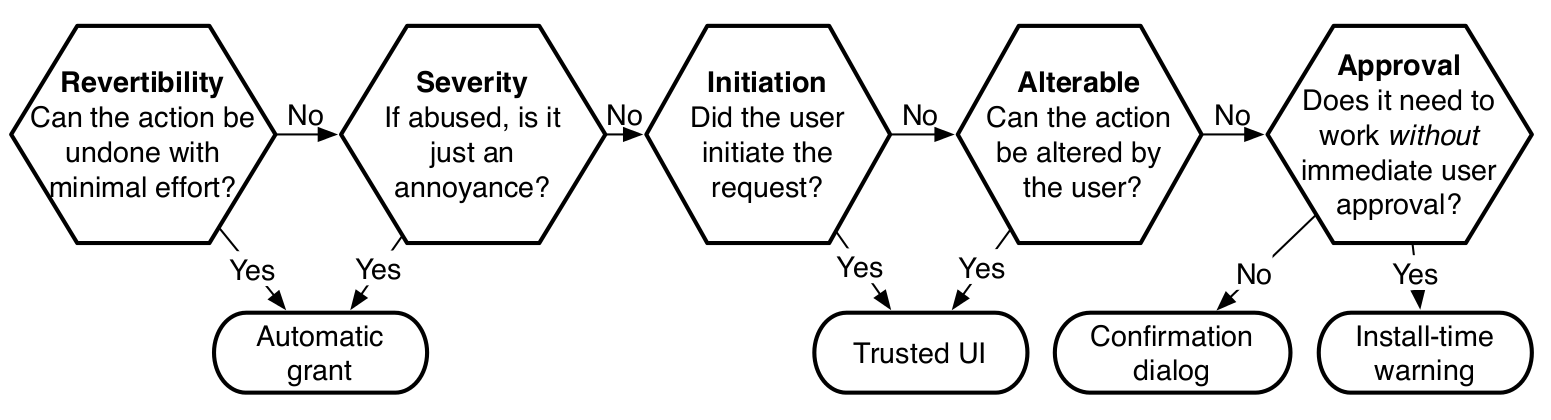
\includegraphics[scale=0.2]{adrienne.png}
  \end{block}
\end{frame}



\begin{frame}
\frametitle{Permission Requests (are totally offtopic)}

	\begin{block}{You have 2 seconds per UI! No more!}
	\begin{itemize}
	\item Don't expect rational decisions, rely on interaction cost instead
	\item Make it useful and actionable
	\item Identify who is asking for permission
	\item Visualise what is asked for
	\end{itemize}
	\end{block}

	{\scriptsize\color{xorg-palette-dark}[Reeder, 2011 on NEAT warnings, Day, 2014 on sandboxing]}

	\begin{important}
	Good design is DE-dependant. No infrastructure work needed in Wayland for permission UIs.
	\end{important}

\end{frame}



\begin{frame}
\frametitle{\circled{\large{3}} Authentication UIs}

\begin{block}{Spoofing Auth UIs is highly rewarding... and easy}
	\begin{columns}[T]
		\begin{column}{0.6\paperwidth}
			\begin{itemize}
			\item Just fake the \texttt{polkit} UI!
			\item Or go fullscreen and fake:
				\begin{itemize}
				\item The whole desktop environment
				\item The greeter/lock screen
				\item A Web login page
				\end{itemize}
			\end{itemize}
		\end{column}
		\begin{column}{0.4\paperwidth}
			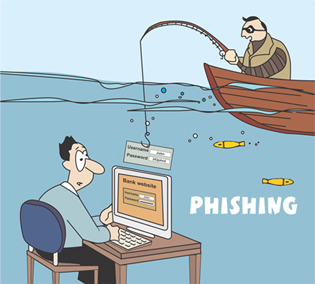
\includegraphics[scale=0.35]{phishing.jpg}\\
			\vskip-.7em\hskip6.5em{\tiny \color{xorg-ppt-warm-grey} \copyright ~ Cyberoam}
		\end{column}
	\end{columns}
\end{block}
\end{frame}


\begin{frame}
\frametitle{Please Pwn my Authentication UI}
\centering
\vspace{-0.6em}
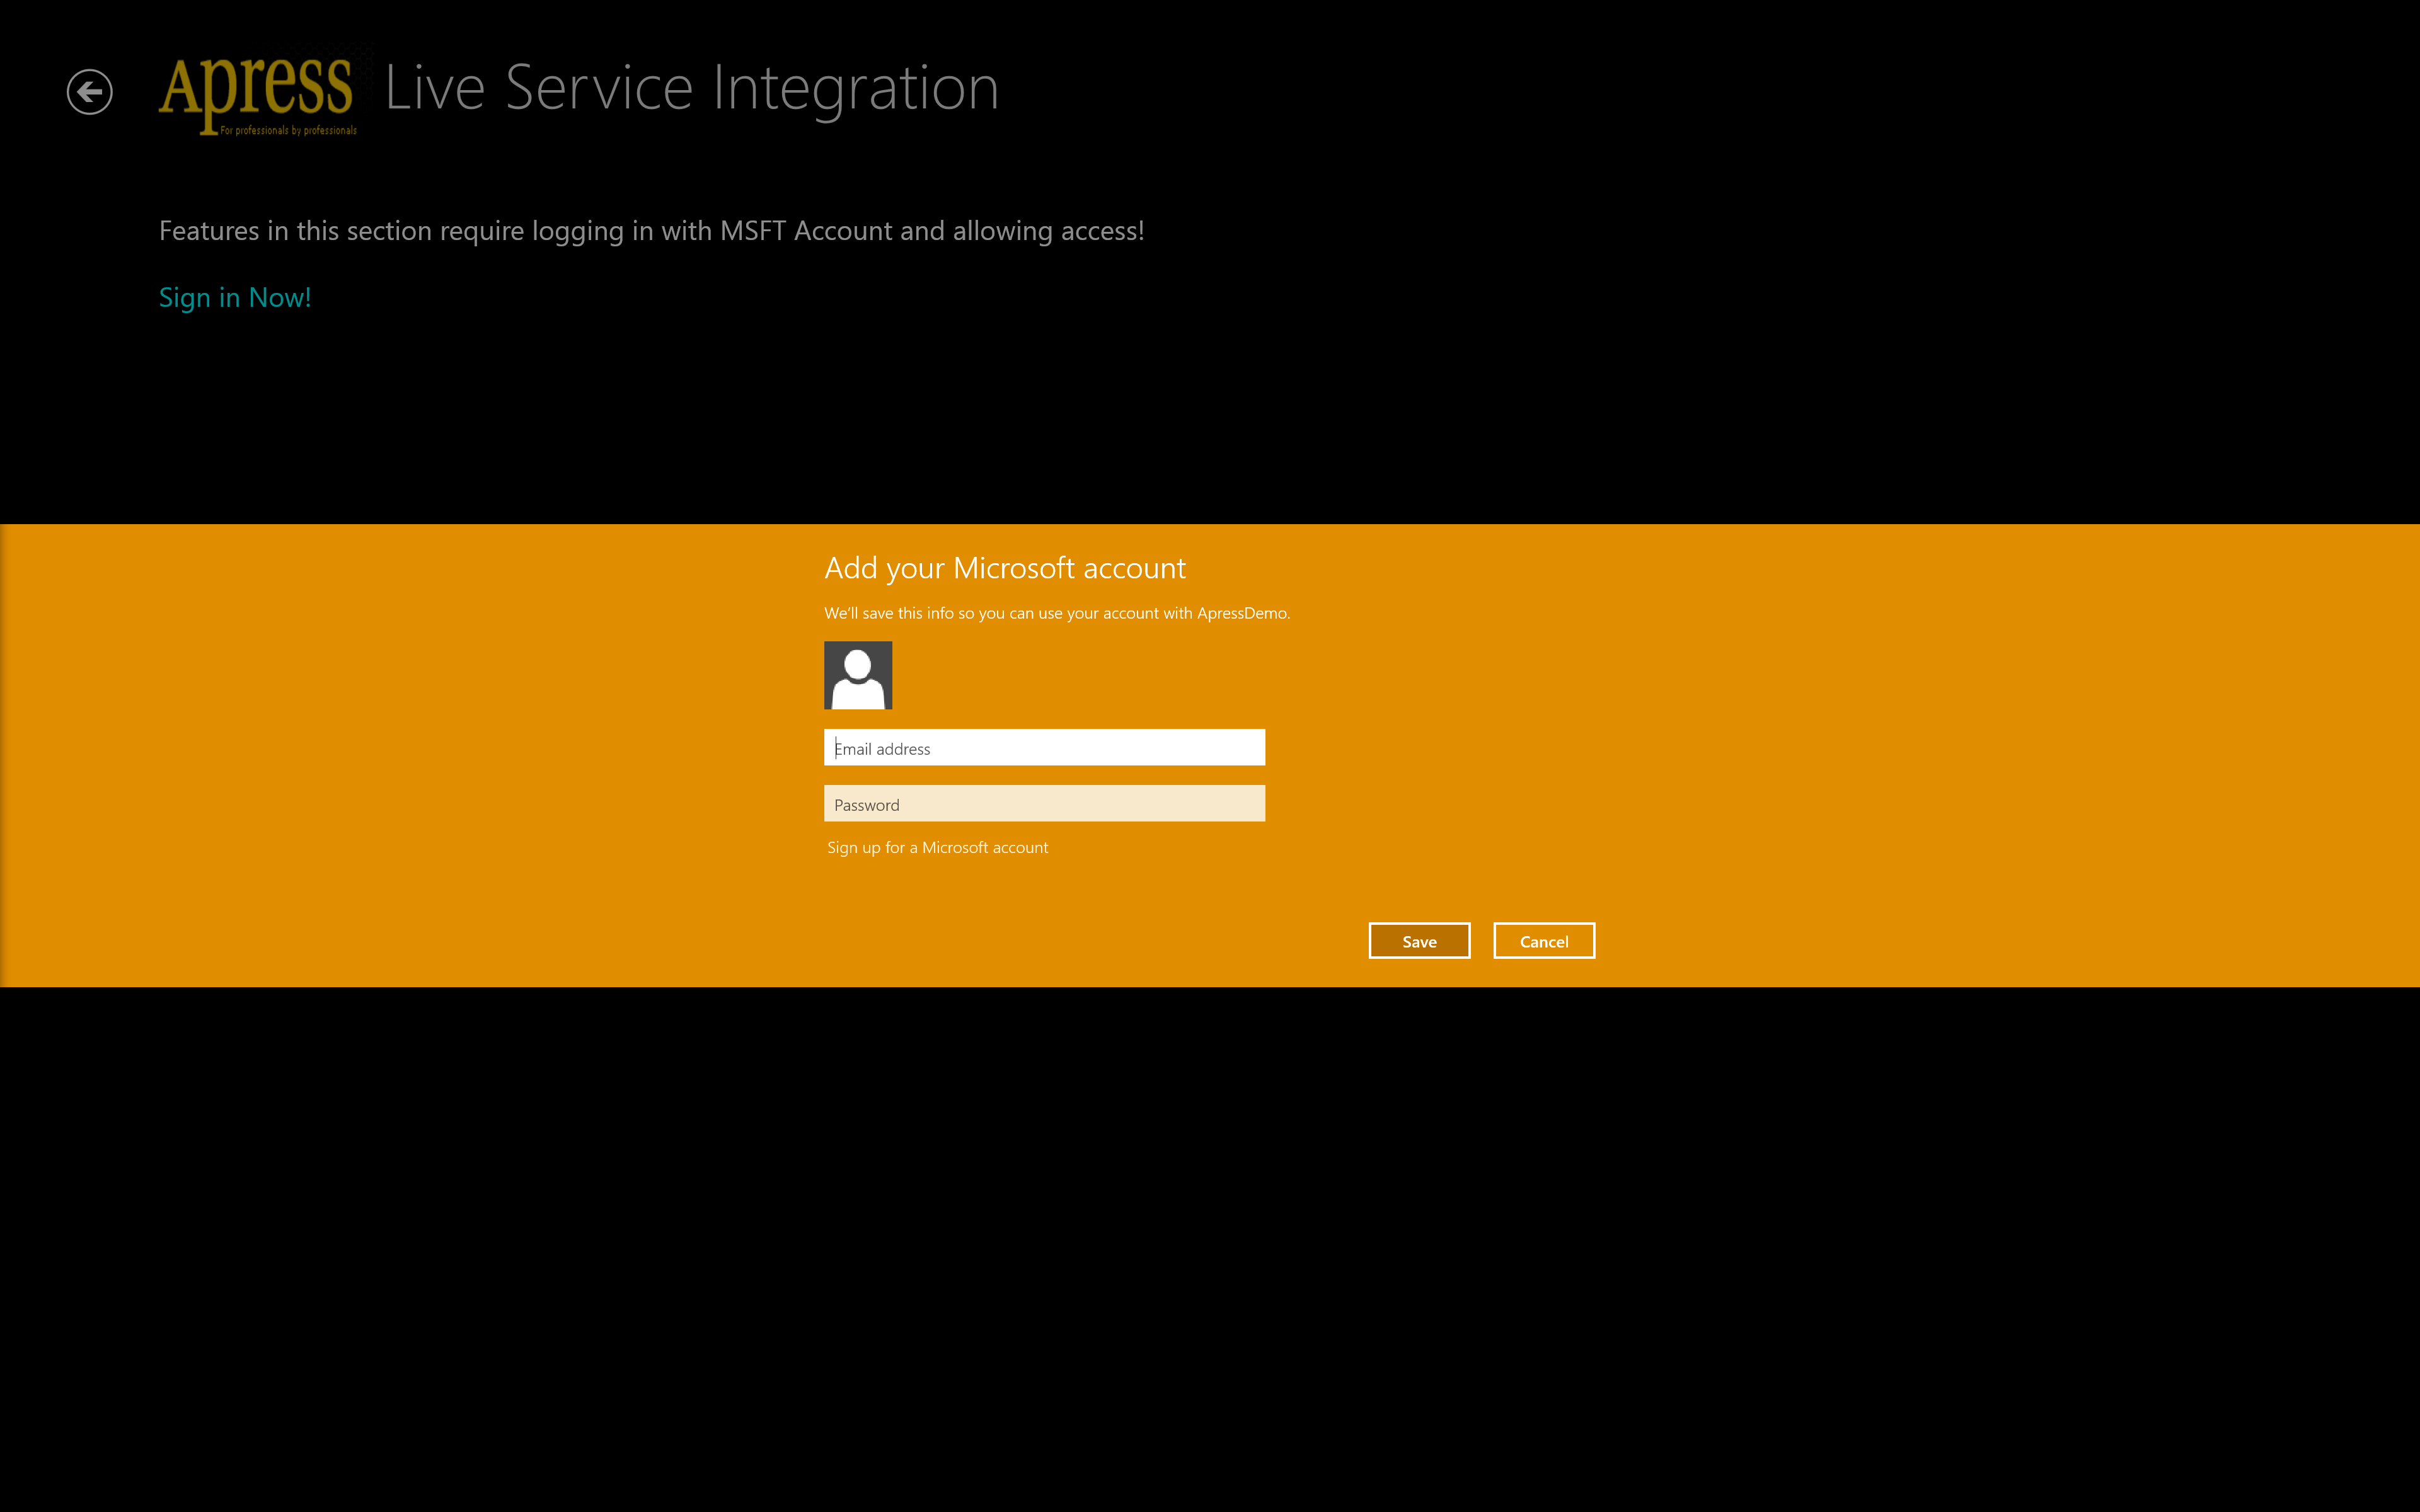
\includegraphics[height=0.9\textheight]{figures/failed-auth.png}
\end{frame}



\begin{frame}
\frametitle{Please Pwn my Authentication UI}

When users open your rogue app's settings, display this:

~

\centering
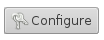
\includegraphics[height=1.5em]{figures/configure-button.png}\\\vskip-0.85em+\\
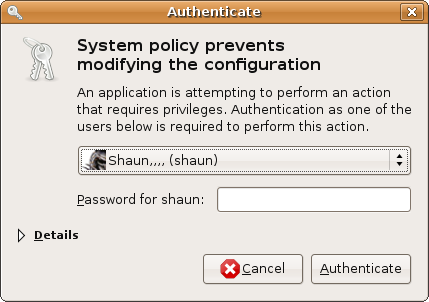
\includegraphics[height=0.4\textheight]{figures/polkit.png}\\
\end{frame}


\begin{frame}
\frametitle{Defences}

	\begin{block}{Three (imperfect) approaches}
		\begin{enumerate}[leftmargin=1.0em]
		\item[Unspoofability] GFX effects only the shell can make
		\item[Indirections] add a user action to all auth (e.g., Windows UAC)
		\item[Mutual Auth] make the DE show the user a secret
		\end{enumerate}
	\end{block}

	\begin{important}
	All three can be broken with a bit of user inattention/confusion.
	\end{important}
\end{frame}


\begin{frame}
\frametitle{Attacking Auth UI Defences}

	\begin{block}{Unspoofable Effects}
		\begin{itemize}
		\item \textit{e.g.}, wobbly animation on background windows
		\item Not trivial to simulate but...
		\item Will users pay attention to the auth dialog or to the background?
		\end{itemize}
	\end{block}

	\begin{block}{Indirections}
		\begin{itemize}
		\item Ctrl+Alt+Del? Bind each key individually and show your fake UI
		\item Or tell the user an error occurred and pop a new UI
		\end{itemize}
	\end{block}

	\textbf{Actual out-of-band communication is necessary!}
\end{frame}


\begin{frame}
\frametitle{Example: "Anti-Phishing" Mutual Auth}

\begin{center}
	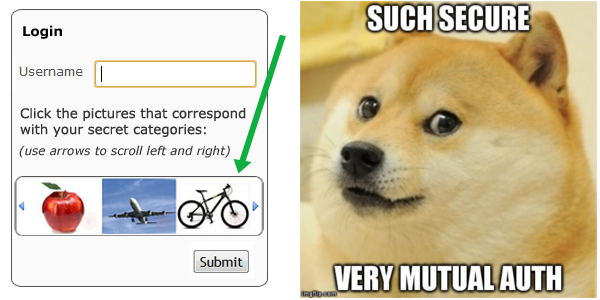
\includegraphics[scale=0.35]{mutual-auth.png}\\
	\vskip-.7em\hskip-7em{\tiny \color{xorg-ppt-warm-grey} \copyright ~ Confident Technologies}
\end{center}

	\begin{important}
	Tell users ``The image server is down'' and they all proceed!\par~\\
	\textbf{Lesson:} cultural context matters. Errors expected on the Internet
	\end{important}
\end{frame}




\section{Conclusion}
\begin{frame}
\frametitle{Thanks for your Attention!}

  \begin{block}{What we have}
  \begin{itemize}
  \item A LibWSM prototype to enable privileged interfaces
  \item Open problems for security UIs design
  \item More detailled versions on \url{mupuf.org/blog}
  \end{itemize}
  \end{block}

  \begin{columns}[T]
    \begin{column}{0.6\paperwidth}
	  \begin{block}{What comes next}
		\begin{itemize}
		\item Martin to finish and maintain LibWSM
		\item Steve to study Linux users' security practices in-the-wild
		\item All of us to review privileged APIs?
		\end{itemize}
	  \end{block}
    \end{column}
    \begin{column}{0.3\paperwidth}
      \vspace{1.5em}
      \color{xorg-palette-dark}
      \hspace{6em}
\includegraphics[scale=0.4]{octopi.png}
      \vspace{-1em}
      \rule{.29\paperwidth}{1pt}
      \vskip0.1em
      \scriptsize
        \usebeamerfont{author}\color{xorg-palette-dark}\insertshortauthor
        \color{xorg-slide-fg}\insertaddress

      \vskip1em
      \scriptsize
        \color{xorg-palette-dark}\insertinstitute \\
        \color{xorg-slide-fg}\insertemail \\

      \vskip-0.3em
      \color{xorg-palette-dark}
      \rule{.29\paperwidth}{1pt}
      \vskip0.5em
    \end{column}
  \end{columns}

%    Create scenarii for security breakdowns/resolutions
%    Let people use devices over months, see what issues they encounter
%    Simulate privacy/security violations, observe responses
%    Evaluate the experience of people, not the ``usability'' of UIs in a lab
\end{frame}

